\documentclass[onecolumn,10pt,titlepage]{article}
\usepackage[a4paper,top=2.5cm,bottom=2cm,left=2cm,right=2cm,marginparwidth=1.75cm,headheight=28pt]{geometry}
% Formateo para castellano
\usepackage[utf8]{inputenc}
\usepackage[spanish,mexico]{babel}

%Bibliografía
\usepackage{natbib}
% Simbolos para notas de pie
\usepackage[symbol]{footmisc}
\renewcommand*{\thefootnote}{\fnsymbol{footnote}}

% \renewcommand{\thefootnote}{\fnsymbol{footnote}}
% \footnote[num]{text}

% \pagestyle{myheading}
% \markright{Mi Documento \hfill Mi nombre \hfi}
%
\usepackage{fancyhdr,framed}
\setlength{\headheight}{15.2pt}
\pagestyle{fancy}
\lhead{Elementos Finitos II - 31.92 \\ Patricio Whittingslow -- 55423}
\chead{TP 1}


%\usepackage{subcaption}

% Para el entorno align
\usepackage{amsmath}

% Multiples columnas para glosario
\usepackage{multicol}

%Figuras y subtitulos
\usepackage{graphicx}
\usepackage{caption,subcaption}
\usepackage{hyperref}
\hypersetup{
    colorlinks,
    citecolor=black,
    filecolor=black,
    linkcolor=black,
    urlcolor=black
}

%Helvetica
\renewcommand{\familydefault}{\sfdefault}
\usepackage[scaled=1]{helvet}
\usepackage[format=plain,
            labelfont={bf,it},
            textfont=it]{caption}
%--------------------------------------



\usepackage{siunitx}
\newcommand{\glossentry}[2]{$#1$ \indent #2 \par \vspace{.4cm} }
\newcommand{\adm}{\textrm{adm}}

%\newcommand{\unit}[1]{\textsf{#1}}
%\newcommand{\mega}{\unit{M}}
%\newcommand{\milli}{\unit{m}}
%\newcommand{\giga}{\unit{G}}
%\newcommand{\meter}{\unit{m}}
%\newcommand{\pascal}{\unit{Pa}}
%\newcommand{\kilo}{\unit{k}}
%\newcommand{\si}[1]{#1}
%\newcommand{\SI}[2]{#1\si{#2}}
\title{Informe Técnico - ITBA}

\author{Patricio Whittingslow}
%========================> Comienza Documento
\begin{document}
\begin{titlepage}
	\centering
	
	{ \large Instituto Tecnológico de Buenos Aires  \par }
	\vspace{2cm}
	{\Large \scshape Elementos Finitos II - 31.92 \par}
	\vspace{2cm}
	{\Huge \scshape Estudio del Doble Fondo de un Buque\par }
	\vspace{.5cm}
	{\Large Y un estudio de placas preliminar \par}
	\vspace{2cm}
	{\large \bf Autor \par}
	\vspace{.5cm}
	\textsc{\large Patricio Whittingslow -- 55423}
	\vspace{2cm}
	{\par \large Fecha de realización: \today \par}
	\vspace{1cm}
	{\large Fecha de entrega: .......................................\par}
	\vspace{2.5cm}
	{\large Firma del docente: .......................................}
	\vspace{3cm}
	\begin{figure}[htb!]
		\centering
		
\includegraphics[width=6cm]{fig/logoitba.png}
	\end{figure}
\end{titlepage}


{\textbf{Problema}}\par
Se estudia la estructura de la base de un buque empleando el uso del método de elementos finitos. Las hipótesis empleadas son de desplazamientos pequeños y material isótropo.

\begin{multicols}{2}
	\section*{Glosario}
	\glossentry{F}{Rigidez ante la flexión.}
	\glossentry{p}{Carga de presión.}
	\glossentry{\kappa_{0}}{Curvatura de placa inicial.}
\end{multicols}


\tableofcontents


\section{Introducción Teórica}
Se opta por resolver el problema con elementos cascaras de 4 nodos y elementos vigas. Antes de comenzar a modelar se estudió el funcionamiento de los elementos placas (Mindlin y Kirchoff) para tener un concepto fundado de como se pueden emplear y cual es su comportamiento ante casos empotrados y articulados.

En el estudio de cascaras con pequeñas deformaciones en general toma en cuenta las siguientes suposiciones\cite{ugural2003advanced}

\begin{enumerate}
	\item La relación entre el espesor de la cascara al radio de curvatura es mucho menor a la unidad
	\item Desplazamientos son muy pequeños en comparación con el espesor
	\item Secciones rectas de un elementos, perpendiculares al plano medio, permanecen rectas y perpendiculares al plano \textit{deformado}.
	\item Se desprecia $\sigma_z$ (al igual que en placas).
\end{enumerate}


Los elementos cascaras tienen la ventaja de poder tomar formas curvas, a diferencia de los elementos placas. Las tensiones en las cascaras (\ref{eq:cascaras}) varían de forma lineal a lo largo del espesor y a la vez estas tensiones son inversamente proporcional al espesor \citep{cook2007concepts}.\\
\begin{equation} \label{eq:cascaras}
\sigma_{x}=\frac{N_{x}}{t}+\frac{M_{x} z}{t^{3} / 12} \qquad \sigma_{y}=\frac{N_{y}}{t}+\frac{M_{y} z}{t^{3} / 12} \qquad \tau_{x y}=\frac{N_{x y}}{t}+\frac{M_{x y} z}{t^{3} / 12}
\end{equation}

Los elementos placas tienen similitudes. Las tensiones también (salvo el corte en $zx$) varían de forma lineal, pero a diferencia de las cascaras, las tensiones son exclusivamente inversamente proporcionales al cubo del espesor. No era el caso para las tensiones axiales de $N_x,N_y$ y $N_{xy}$ de las cascaras. Para placas \citep{ugural2003advanced}:

\begin{align} \sigma_{x} &=\frac{E}{1-v^{2}}\left(\varepsilon_{x}+v \varepsilon_{y}\right)=-\frac{E z}{1-v^{2}}\left(\frac{\partial^{2} w}{\partial x^{2}}+v \frac{\partial^{2} w}{\partial y^{2}}\right) \label{eq:sigxplacas}\\ \sigma_{y} &=\frac{E}{1-v^{2}}\left(\varepsilon_{y}+v \varepsilon_{x}\right)=-\frac{E z}{1-v^{2}}\left(\frac{\partial^{2} w}{\partial y^{2}}+v \frac{\partial^{2} w}{\partial x^{2}}\right) \\ \tau_{x y} &=\frac{E}{2(1+v)} \gamma_{x y}=-\frac{E z}{1+v} \frac{\partial^{2} w}{\partial x \partial y} 
\end{align}
donde las segundas derivadas parciales de los desplazamientos se relacionan al espesor según la constitutiva \ref{eq:constitutive}

\begin{equation} \label{eq:constitutive}
\left\{\begin{array}{l}{M_{x}} \\ {M_{y}} \\ {M_{x y}}\end{array}\right\} =- \left[ \begin{array}{ccc}{F} & {\nu F} & {0} \\ {\nu F} & {F} & {0} \\ {0} & {0} & {\frac{(1-\nu) F}{2}}\end{array}\right] \left(\left\{\begin{array}{l}{w_{,x x}} \\ {w_{,y y}} \\ {2 w_{,x y}}\end{array}\right\}-\left\{\kappa_{0}\right\} \right)
\end{equation}

donde $F=\frac{E t^{3}}{12\left(1-\nu^{2}\right)}$ es la rigidez ante la flexión. Resulta aparente ahora que dado un momento sobre la placa (Siendo la curvatura inicial igual a cero) la placa se curvará con un radio proporcional a $1/t^3$. Esta curvatura luego definirá las tensiones vistas en \eqref{eq:sigxplacas}. 

\section{Estudio con placas planas}
Las placas analizadas son Kirchoff, Mindlin Q4 y Mindlin Q8.

\subsection{Método}
El problema trata una placa de espesor $t$ con dimensiones $a\times b$ donde $a=1,4\si{\meter}$ y $b=1\si{\meter}$. El material es acero\footnote{$E=\SI{210}{\giga \pascal}$ y $\nu=0,3$}. Los casos son con presión uniforme $p$ para los espesores $t=a$, $t=\frac{a}{10}$ y $t=\frac{a}{100}$. El factor de corrección para tensión por corte transverso es igual a $k=\frac{5}{6}$ usando integración selecta\citep{cook2007concepts} para placas Mindlin.

Se tiene que para una placa simplemente apoyada con carga uniforme el desplazamiento máximo esta dada por \citep{ugural2003advanced}
\begin{equation}\label{eq:uguralwmax}
w_{\max }=\frac{16 p}{\pi^{6} F} \sum_{m}^{\infty} \sum_{n}^{\infty} \frac{(-1)^{\frac{m+n}{2}-1}}{m n\left[(m / a)^{2}+(n / b)^{2}\right]^{2}}\qquad m,n = 1,3,5 \ldots
\end{equation}
el cual nos dará el error.

Por ultimo se estudiaron las tensiones para la placa simplemente apoyada en todos sus lados y para el caso empotrado en todos sus lados.

\subsection{Resultados}
Los resultados se comparan con la solución analítica para una placa simplemente apoyada \eqref{eq:uguralwmax}\footnote{Utilizando $n=m=9$ dado que convergía bien para ese número de iteraciones.}. Para los casos estudiados el desplazamiento máximo es $w_{\max}(t)\approx \SI{6,71e-9}{\meter}$, $w_{\max}(0,1t)\approx \SI{6,71e-6}{\meter}$, $w_{\max}(0,01t)\approx \SI{6,71e-3}{\meter}$. Como sería de esperar, hay una relación del tipo $w(t)=Ct^3$.
\subsubsection*{Caso Empotrado}
La tabla \ref{tab:Convergencia} muestra un estudio de convergencia para los elementos. 
\begin{table}[htb!] 
	\centering
	\begin{tabular}{clll}
		Número de Elementos& Kirchoff & Mindlin Q4 & Mindlin Q8  \\ \hline
		60  & \SI{1,758}{\milli \meter}  &  \SI{1,869}{\milli \meter}  & \SI{1,955}{\milli \meter} \\
		280  & \SI{1,919}{\milli \meter}  &  \SI{1,950}{\milli \meter}  & \SI{1,966}{\milli \meter} \\
		4800 &\SI{1,957}{\milli \meter}  &   \SI{1,965}{\milli \meter} &\SI{1,966}{\milli \meter} \\
		15552 &  \SI{1,959}{\milli \meter}   &  \SI{1,965}{\milli \meter}  & \SI{1,966}{\milli \meter}\\
		21600&  \SI{1,959}{\milli \meter}& \SI{1,965}{\milli \meter}  & \SI{1,966}{\milli \meter}
	\end{tabular}\
	\caption{Desplazamientos máximos para carga uniforme $p=\SI{5}{\kilo \pascal}$ sobre placa \textbf{empotrada} con espesor $t=\frac{a}{100}$. Relación de aspecto de elementos 4:3. Utilizando integración selecta\citep{cook2007concepts}, el más costoso numéricamente por elemento fue Mindlin Q8 por un margen considerable.}
	\label{tab:Convergencia}
\end{table}

\subsubsection*{Caso simplemente apoyado}
El gráfico \ref{fig:errorplacas} muestra el error obtenido para las placas usadas con una variada cantidad de elementos para condiciones de carga/apoyo fijas. Los otros dos gráficos muestran el tiempo de cálculo y el efecto de espesor sobre los elementos Mindlin, \ref{fig:timeplacas} y \ref{fig:espesorplacas} respectivamente. Los elementos Kirchoff no fueron analizados por no prestarse cambios de error graves variando el espesor.

\subsection{Conclusiones}
Los elementos Mindlin Q8 y Kirchoff se prestan a converger rápido y con pocos elementos (figura \ref{fig:errorplacas}). Esto se debe a la gran capacidad de un solo elemento de Kirchoff, permitiendo deformaciones del orden cubico para cada elemento. Los elementos Mindlin Q8 tienen una buena capacidad de captar deformaciones gracias al alto orden de funcionalidad. Los elementos Q4 quedan en tercer lugar. 

De aquí surge la cuestión si es mejor usar elementos Kirchoff o los Q8 para modelar placas planas. Le dirijo la atención al lector a la figura \ref{fig:timeplacas}. Los elementos Kirchoff son costosos desde un punto de vista numérico. La gran ventaja de los elementos Mindlin es la formulación paramétrica que permite una integración rápida por puntos de Gauss. Los elementos Q4 merecen una mención honorable por permitir modelar grandes cantidades de elementos sin impedimento en el tiempo de resolución. 

El espesor es otro factor importante para cuando se tiene que fijar el modelo. No sirve modelar una placa espesa con elementos Mindlin. Sería mejor considerar elementos 3D dado que rápidamente se dispara el error para espesores relativamente pequeños(figura \ref{fig:espesorplacas}). Un espesor $\frac{t}{a}=0.07$ presenta un error relativo de 10\% para el problema estudiado .

Las tensiones son de gran interés para cualquier aplicación de elementos placas. Como vemos en la figura \ref{fig:VM}, los dos casos estudiados presentan diferencias marcadas.  Para la placa empotrada tenemos una curvatura alta en los bordes y menos pronunciada en el centro. Como bien ya sabemos de las ecuaciones \eqref{eq:sigxplacas}, la tensión axíl va mano en mano con dicha curvatura $\frac{\partial^2 w}{\partial x^2}$ y $\frac{\partial^2 w}{\partial y^2}$. Cabe destacar que las mayores tensiones van a estar en los lados mas largos porque son los que precisan girar mayor cantidad en menos distancia para llegar al $w_{\max}$. Por ultimo, se menciona el máximo local de tensiones ubicado en el centro de la placa debido a otro máximo de la suma $\frac{\partial^2 w}{\partial y^2}+\frac{\partial^2 w}{\partial x^2}$.

El caso de una placa simplemente apoyada es bien diferente. Al quedar con giro en sus bordes su mayor curvatura quedaría en el centro. Por ende, también estaría allí la mayor tensión axíl.

\begin{figure}[htb!]
	\centering
	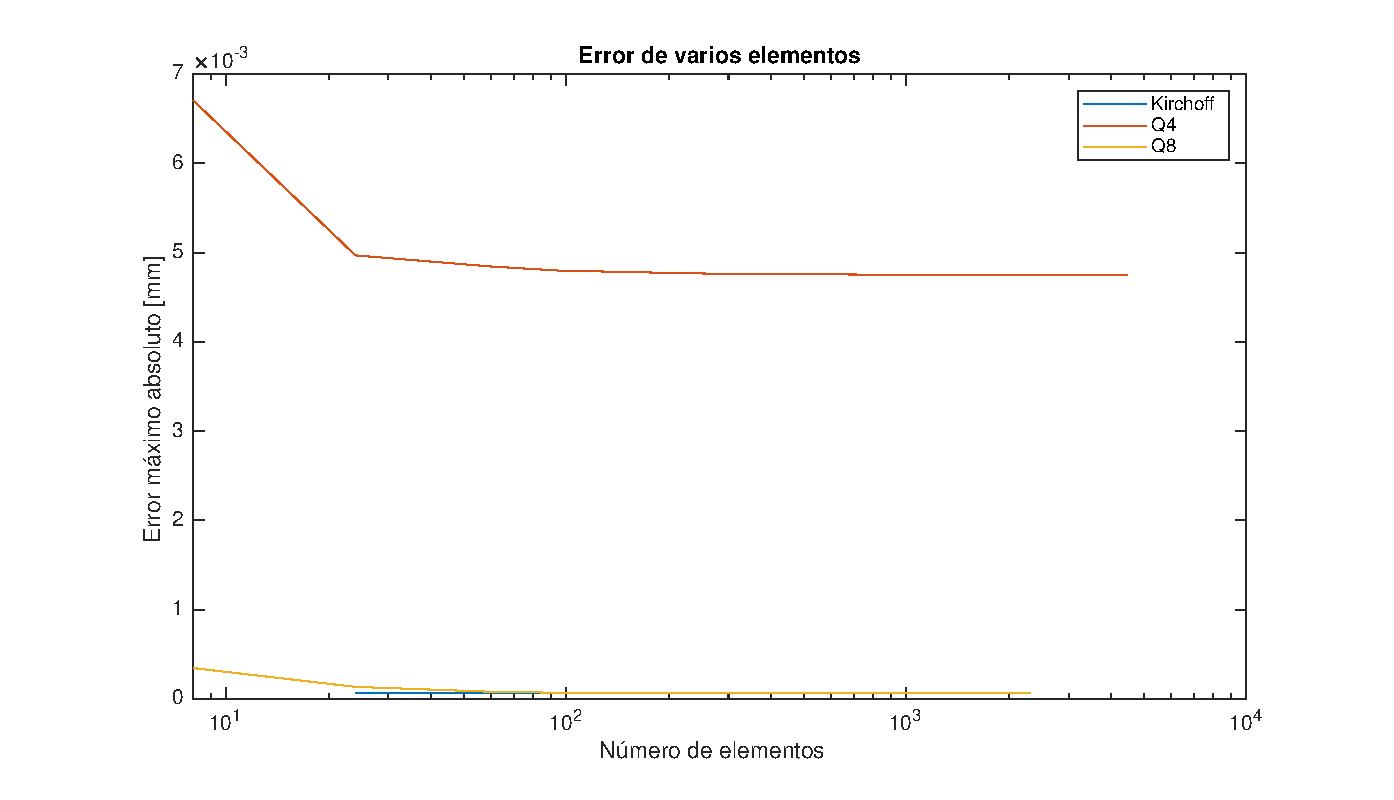
\includegraphics[width=.9\textwidth]{fig/errvec.eps}
	\caption{El error absoluto mejora con el aumento de elementos, desde siempre.}\label{fig:errorplacas}
\end{figure}

\begin{figure}[htb!]
	\centering
	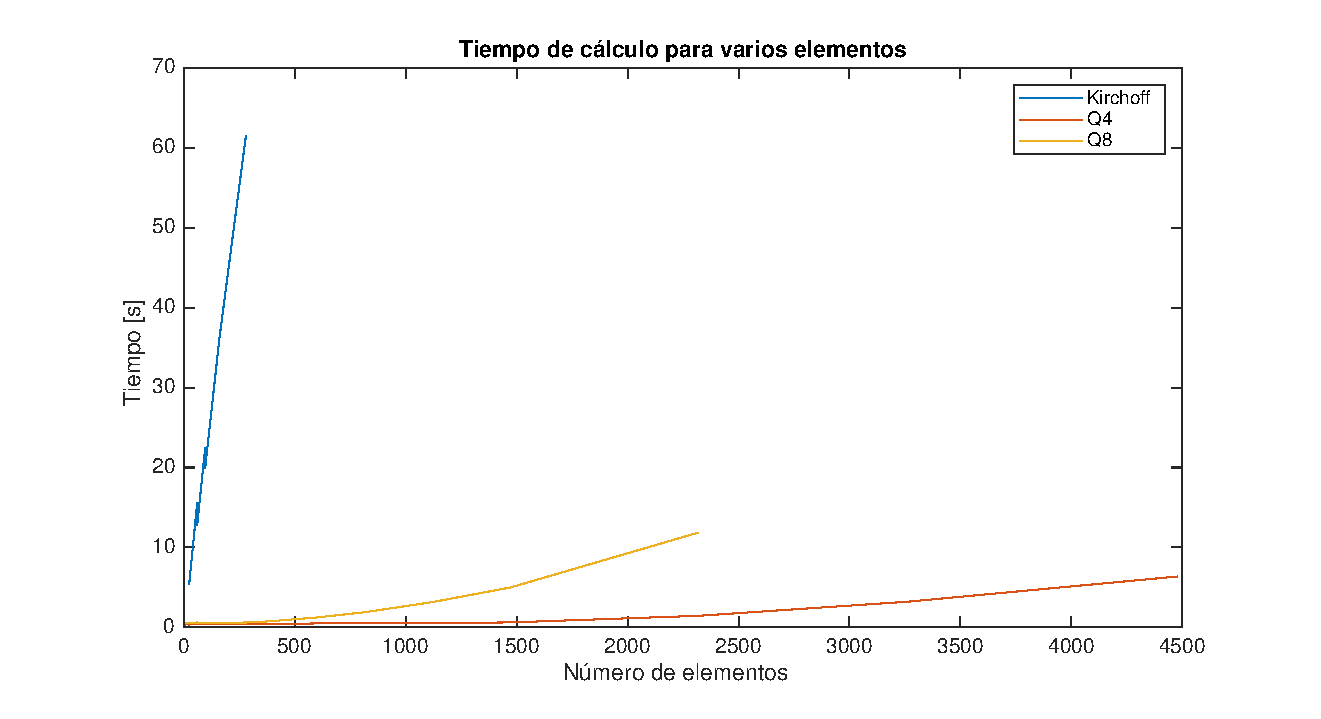
\includegraphics[width=.9\textwidth]{fig/time.eps}
	\caption{El tiempo de cálculo de los elementos tratados. \textbf{Mayor es peor}. Los elementos Kirchoff integrados simbólicamente son los más pesados numéricamente.}
	\label{fig:timeplacas}
\end{figure}

\begin{figure}[htb!]
	\centering
	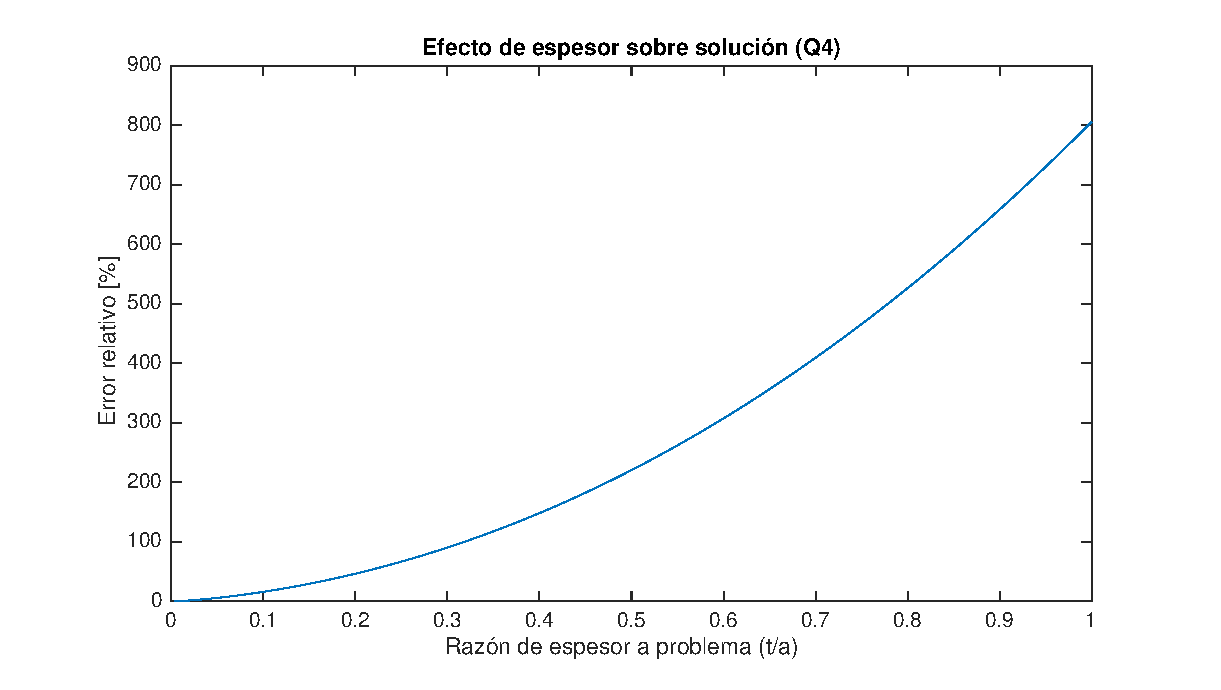
\includegraphics[width=.9\textwidth]{fig/espesor.eps}
	\caption{Relación error relativo máximo vs. espesor para elementos Mindlin Q4. Note que es un gráfico adimensional.}
	\label{fig:espesorplacas}
\end{figure}


\begin{figure}[htb!]
 \centering
 \begin{subfigure}{0.49\textwidth}
 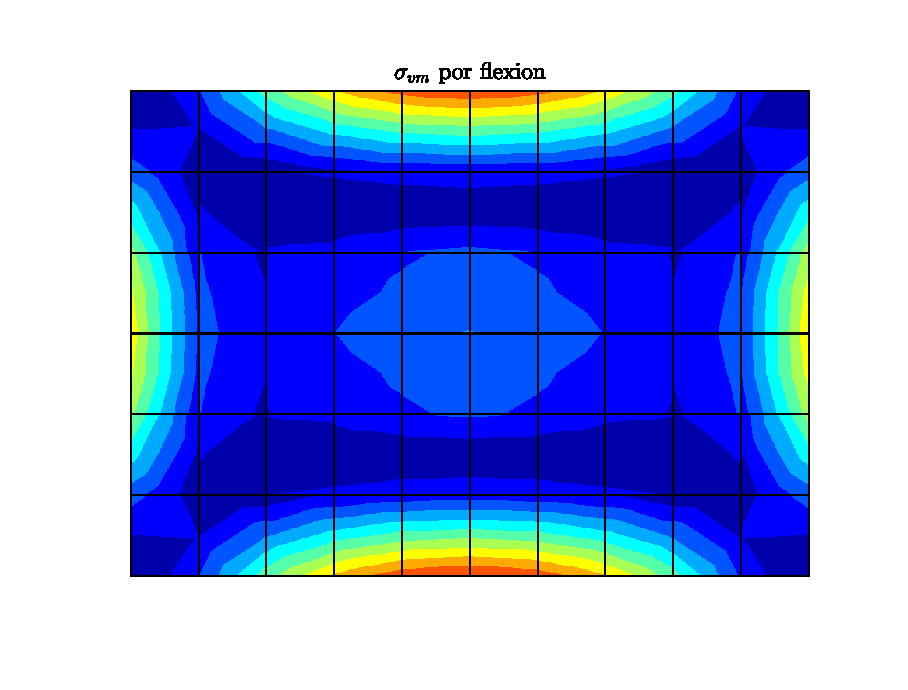
\includegraphics[width=\linewidth]{fig/VM.eps}
 \caption{Caso empotrado}
 \label{fig:VMempotrado}
 \end{subfigure}
 \begin{subfigure}{0.49\textwidth}
 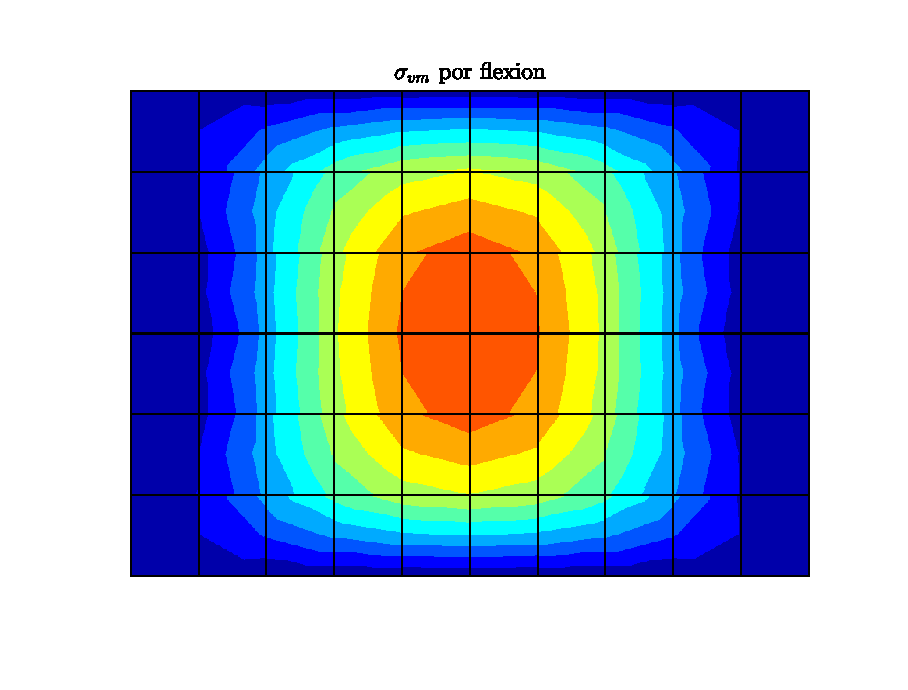
\includegraphics[width=\linewidth]{fig/VMapoyado.eps}
 \caption{Caso simplemente apoyado}
 \label{fig:VMapoyado}
 \end{subfigure}
 \caption{Tensiones calculadas de Von Mises para elementos Q8. Divisiones de elementos visible. Tensiones en Pascales. Se puede observar claramente el comportamiento diferente ante la restricción de giro. Un caso empotrado sufre de flexión en sus bordes mientras que la placa apoyada va fallar por corte.}
 \label{fig:VM}
 \end{figure}

\clearpage
\section{Estudio de doble fondo de un buque}
El buque a estudiar tendrá 5 metros de calado, dándonos una presión sobre el doble fondo de alrededor de $p=5 \si{\kilo \pascal}$. Esta va ser la presión nominal para la cual se va resolver el problema.  El modelo tiene una dimensión longitudinal de 4 claras (distancia entre varengas) y dimensión transversal de una vagra (figura \ref{fig:modeloPlanta}). Las longitudinales van a ser perfiles bulbo $280\times13\si{\milli \meter}$, $300\times 13 \si{\milli \meter}$ para el fondo y el doble fondo, respectivamente. La distancia entre varengas es de $3,25\si{\meter}$ y la distancia entre vagras $4,4\si{\meter}$. Como no se dispones de perfiles bulbo en el programa a usar (NX 11.0 de Siemens) se utilizarán perfiles ``L"{} de características similares. Las dimensiones de los perfiles L se obtuvieron para que los momentos de Inercia $I_z$, $I_y$ sean lo más similares. 


\subsection{Método}
\subsubsection*{Modelo}
La cátedra de la materia sugiere un modelo diferente al tratado. Sugería modelar el espacio desde el plano de una vagra a la próxima considerando un plano de simetría sobre una y considerar apoyos simples sobre la otra. Las varengas también estarían simplemente apoyadas. Se dispone del siguiente dibujo que se destaca por estar en estado de superposición, sobreacotado y subacotado a la vez.

\begin{figure}[htb!]
	\centering
	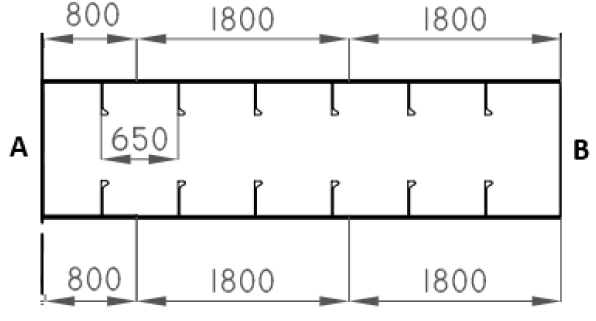
\includegraphics[width=.5\textwidth]{fig/modelocatedra.png}
	\caption{Modelo dado en el enunciado del TP. \textbf{No es el modelo resuelto.} Apoyo simple sobre el plano B, simetría sobre A (ambas son vagras). Apoyos simples sobre varengas.}
	\label{fig:modelocatedra}
\end{figure}
El autor optó por adaptar el modelo comenzando por la normalización de las dimensiones. La figura \ref{fig:modeloTransversal} muestra el corte transversal del modelo tratado. Las condiciones de borde que antes se ubicaban sobre las vagras ahora están en el espacio entre vagras. Esto no debería considerarse más que un cambio estético, ya que matemáticamente ambas estructuras son equivalentes si se emplea la simetría de forma correcta.
\begin{figure}[htb!]
	\centering
	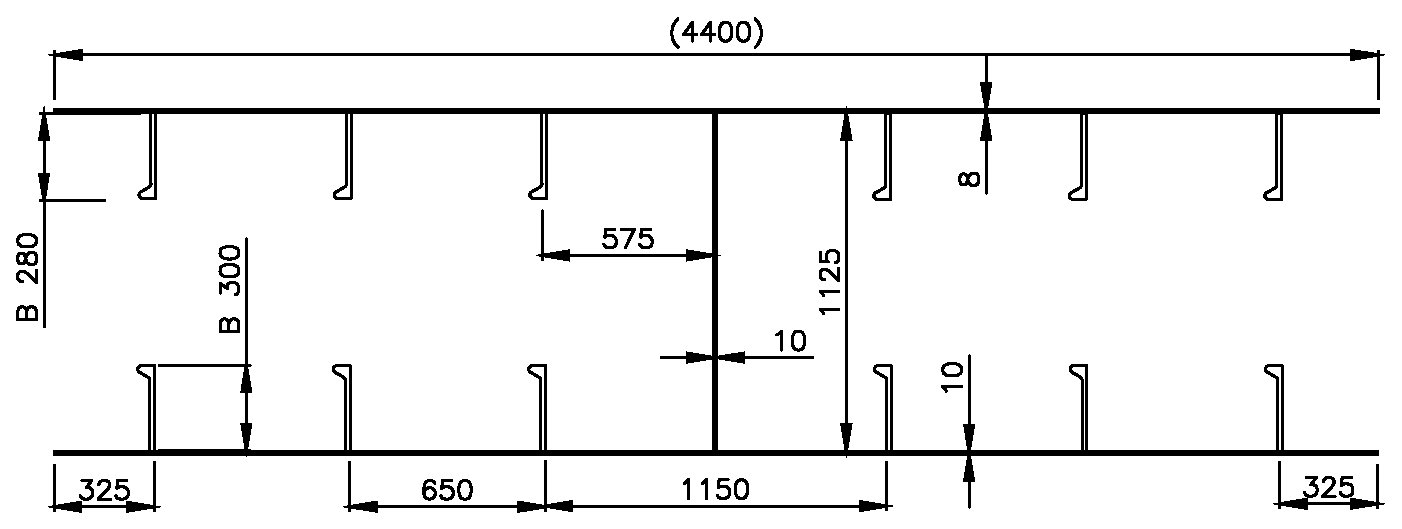
\includegraphics[width=0.7\linewidth]{fig/MODELO.eps}
	\caption{Corte transversal del modelo. La placa superior es el fondo y por el medio queda la vagra. Dimensión longitudinal del modelo es \SI{13,0}{\meter}.}
	\label{fig:modeloTransversal}
\end{figure}

Otros incisos del enunciado:
\begin{itemize}
	\item Realizar un modelo de elementos finitos para la estructura del doble fondo considerando 4 claras (distancia) de varengas
	\item Las varengas límites de la estructura están simplemente apoyadas
\end{itemize}
La interpretación más lógica del segundo inciso es modelar la estructura con dos varengas como tapas, cuyas superficies estén simplemente apoyadas, pues si hablará de apoyar los extremos de las varengas estaría rompiendo la simetría sobre una de las vagras. Sin embargo, un lector astuto tal vez se de cuenta que dados los incisos estos, hay otro plano de simetría diferente al de la vagra. Este plano es transversal al modelo y estaría en la linea media entre las dos varengas límites de la estructura. Aplicar simetría resultaría en un modelo de solo dos claras, una \textbf{clara} violación al enunciado.

El autor entonces modifica el modelo, otra vez cambiando los límites de la estructura propuesta. Los límites transversales ahora se encuentran sobre la linea media entre dos varengas. Estas modificaciones permiten ver dentro del modelo cuando se obtiene una solución, dando paso a la rápida iteración de secciones. También se presta a menor confusión al momento del mallado al otorgar espesor a las varengas/vagras, pues no hay que dividir ningún espesor de placa por dos \citep{cook2007concepts} puesto que no hay planos de simetría que cortan nuestras placas.

Se reitera que las dos estructuras son equivalentes. En este trabajo práctico se va tratar solo \textbf{una.}

\subsubsection*{Condiciones de Borde} 

Se planteo un modelo aprovechando el eje longitudinal simétrico y considerando simetría transversal. Cabe destacar que debido a esta última consideración puede haber discrepancia entre la realidad y lo que se plantea. Es decir, \emph{considerar simetría sobre un eje transversal tomando en cuenta solo 4 claras de distancia es una decisión valida si los esfuerzos se normalizan en magnitud acercándose al borde sin soporte en $z$.\footnote{Se explica a que se refiere con el borde sin soporte en $z$ a continuación.} Caso contrario se debería tomar aún más claras para ver las tensiones mayores que se pueden llegar a alcanzar.}

\begin{figure}[htb!]
	\centering
	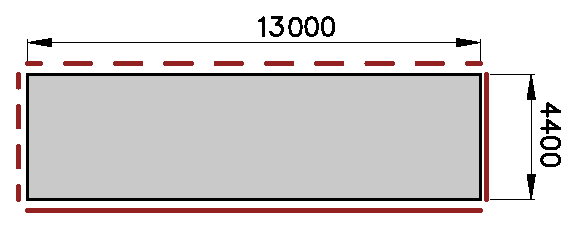
\includegraphics[width=.6\textwidth]{fig/modelnx.eps}
	\caption{Vista en planta del modelo trabajado. Linea punteada representa condiciones de borde de simetría según \citep{cook2007concepts}. Linea solida representa condición de borde especial, idéntica a la simetría con soporte agregado en $z$ (saliente a la hoja).}
	\label{fig:modeloPlanta}
\end{figure}


La simetría es aplicada de forma que se vean esfuerzos generados por el equilibrio entre las dos fuerzas predominantes en un buque, el peso y la presión hidrostática. Para lograr esto se aplican condiciones de borde de simetría en todos los bordes del modelo y una condición especial en un borde transversal y otro longitudinal. La condición a aplicar es un soporte en la dirección de la gravedad, en este caso, un soporte en $z$. Esto dará luz al efecto ``reacción"{} del peso propio del buque ante la presión hidrostática.


\subsection{Resultados y optimización}
Debido a la acción ondulatoria de las olas\footnote{Conocido como esfuerzos de quebranto/arrufo.} el buque en realidad puede ser sometido a una presión aún mayor, por eso se va tomar un factor de seguridad $n=3$ para optimizar.

La gran ventaja del método elementos finitos es el rápido prototipado y obtención de resultados. En meros minutos de modificar las dimensiones del sistema en cuestión el usuario se puede hacer una idea de la relación entre dimensiones y tensiones.

Para el sistema en cuestión se observó que el espesor de vagra del modelo no era determinante para las tensiones globales. En cambio modificar las varengas tiene un efecto amplio ya que no reparten la carga con otros refuerzos como la vagra, así afectando las tensiones del resto del problema. Con esto en mente no es sorpresa porque las vagras mantuvieron su espesor inicial llegado el final de la optimización.

Como se puede ver, los esfuerzos se regularizan al acercarse al borde transversal sin soporte en $z$, lo cual nos da una idea que la situación vista en la figura \ref{fig:2a} podría estar ocurriendo en el interior de un buque. Lo que puede llegar a llamar la atención es que las tensiones son relativamente bajas en los longitudinales.

 \begin{figure}[htb!]
 \centering
 \begin{subfigure}{0.49\textwidth}
 % \begingroup
 \begin{framed}
 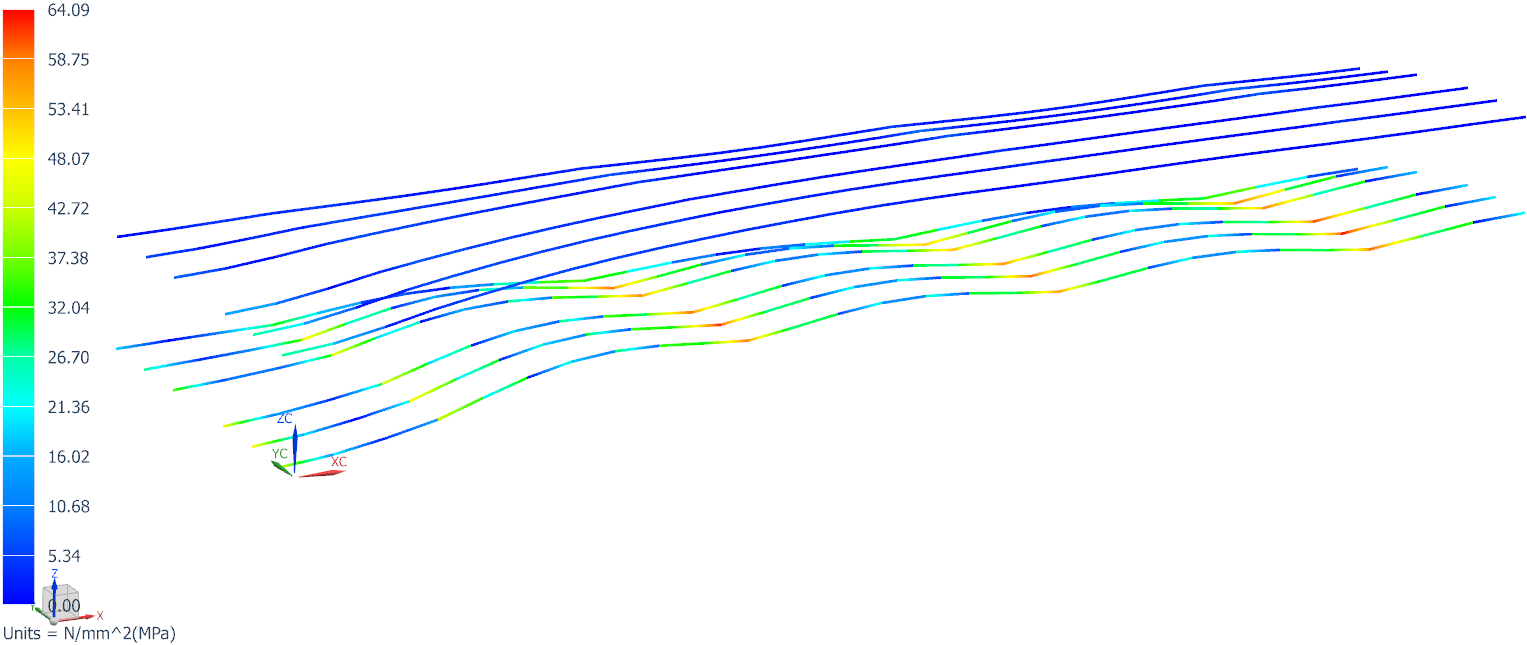
\includegraphics[height=3.3cm,draft]{fig/longitudinales_a.png}
 \caption{Vista de los elementos viga. Perfiles superiores son los $280\times 13\si{\milli \meter}$. $\sigma_{vm_{\max}}= 64,09 $\si{\mega \pascal}.}
 \label{fig:longitudinalesCasoA}
 \end{framed}
 % \endgroup
 \end{subfigure}
 \begin{subfigure}{0.49\textwidth}
 \begin{framed}
 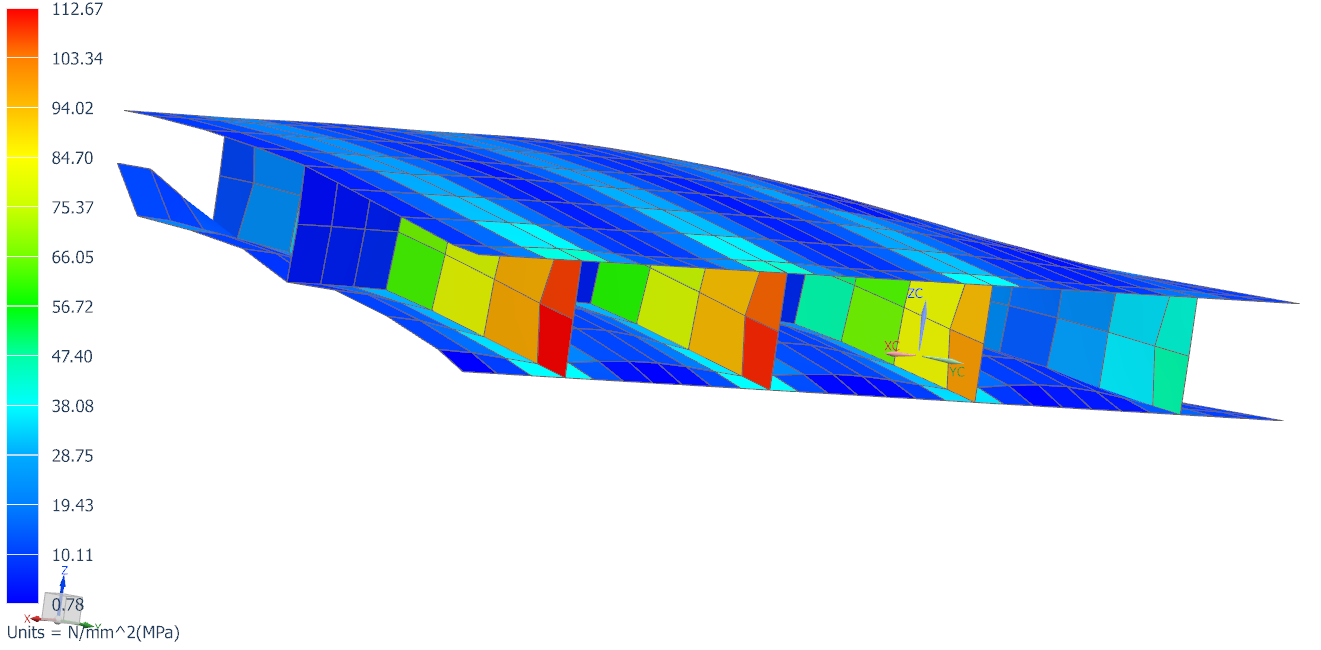
\includegraphics[height=3.3cm,draft]{fig/varengas_a.png}
 \caption{Vista de los elementos cascaras del doble fondo. $\sigma_{vm_{\max}}= 112,67 $\si{\mega \pascal}.}
 \label{fig:VarengasCasoA}
 \end{framed}
 \end{subfigure}
 \caption{Tensiones máximas Von Mises en \si{\mega \pascal}.}
 \label{fig:2a}
 \end{figure}

\subsubsection*{Proceso de optimización}
El material a usar para todos los elementos es el acero AISI 4340 \emph{annealed} con una tensión admisible de \SI{470}{\mega \pascal}.

El proceso de optimización fue iterativo, cambiando los espesores de las vagras, varengas y fondos hasta que todos tengan una zona que este cerca de $\sigma_{\adm}=\frac{\sigma_{y}}{n}\approx\SI{150}{\mega \pascal}$. También se redujeron las secciones de las longitudinales.
\begin{itemize}
	\item $t_{\textrm{vagras}}=\SI{5}{\milli \meter}$
	\item $t_{\textrm{varengas}}=\SI{10}{\milli \meter}$
	\item $t_{\textrm{fondo}}=\SI{4}{\milli \meter}$
	\item $t_{\textrm{doble fondo}}=\SI{7}{\milli \meter}$
	\item Bulbos del fondo $280\times 13$\si{\milli \meter}
	\item Bulbos del doble fondo $260\times 13$\si{\milli \meter}
\end{itemize}

En la figura \ref{fig:optimizacion} se puede observar que las secciones quedaron dimensionadas de forma que la tensión ronde la zona amarilla alrededor de \SI{130}{\mega\pascal}. Existen zonas rojas que superan la tensión admisible, pero estas son singularidades y no deberían ser consideradas para el diseño.

 \begin{figure}
     \centering
     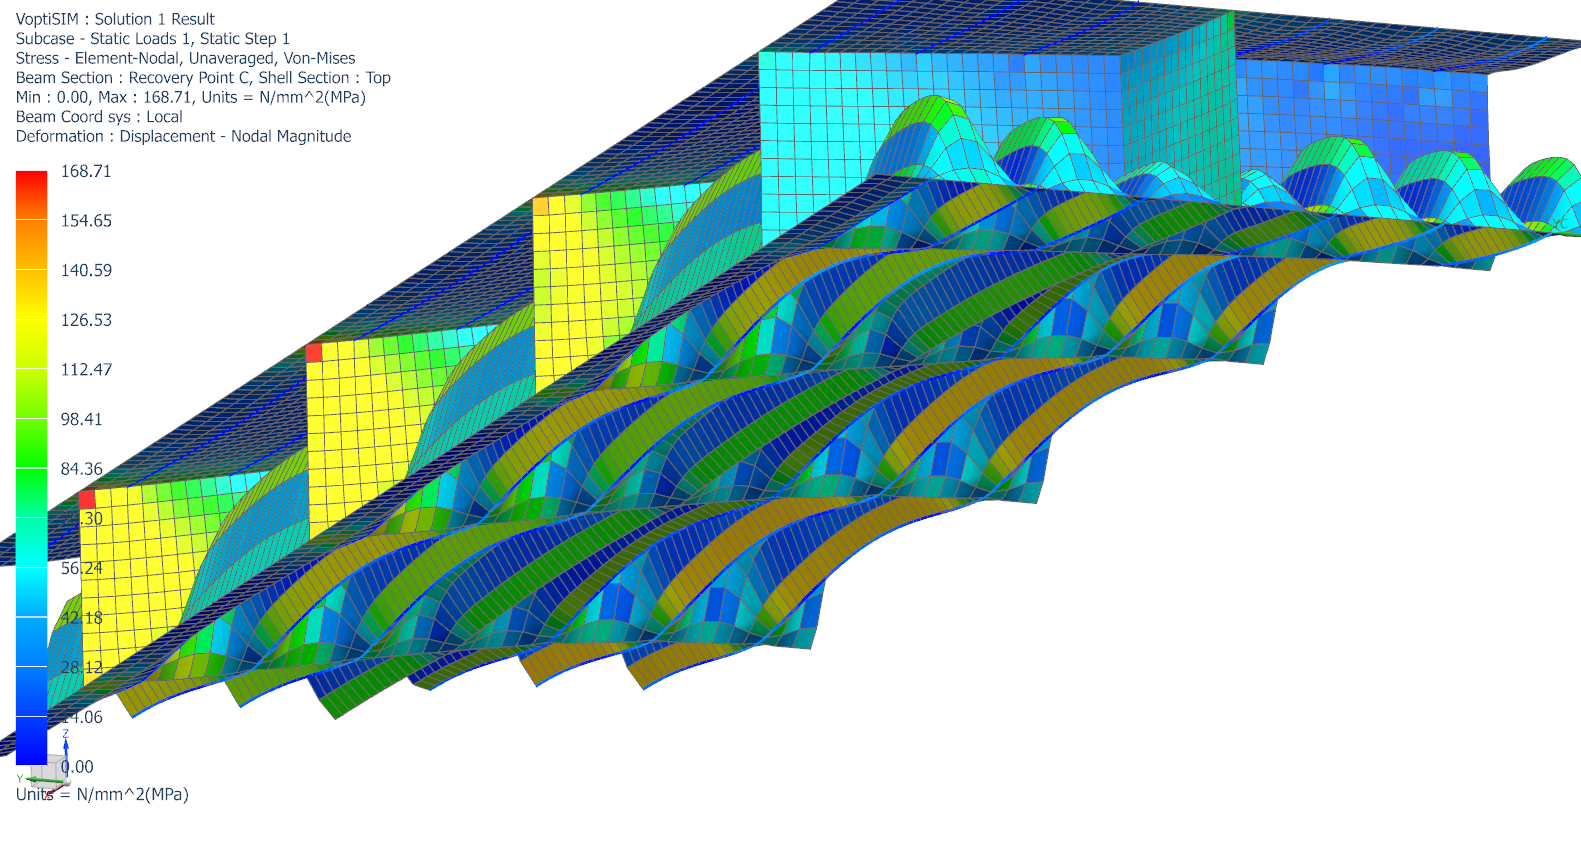
\includegraphics[width=11cm]{fig/VoptiSIM.png}
     \caption{Tensiones son las de Von Mises del resultado final de la optimización.}
     \label{fig:optimizacion}
 \end{figure}

\subsubsection*{Curvas de Schade}
H. A. Schade ha publicado una serie de curvas indicativas de desplazamiento bajo carga uniforme en función de varios parámetros para placas reforzadas. Por la simetrías usadas se duplican las dimensiones.
\begin{figure}[htb!]
	\centering
	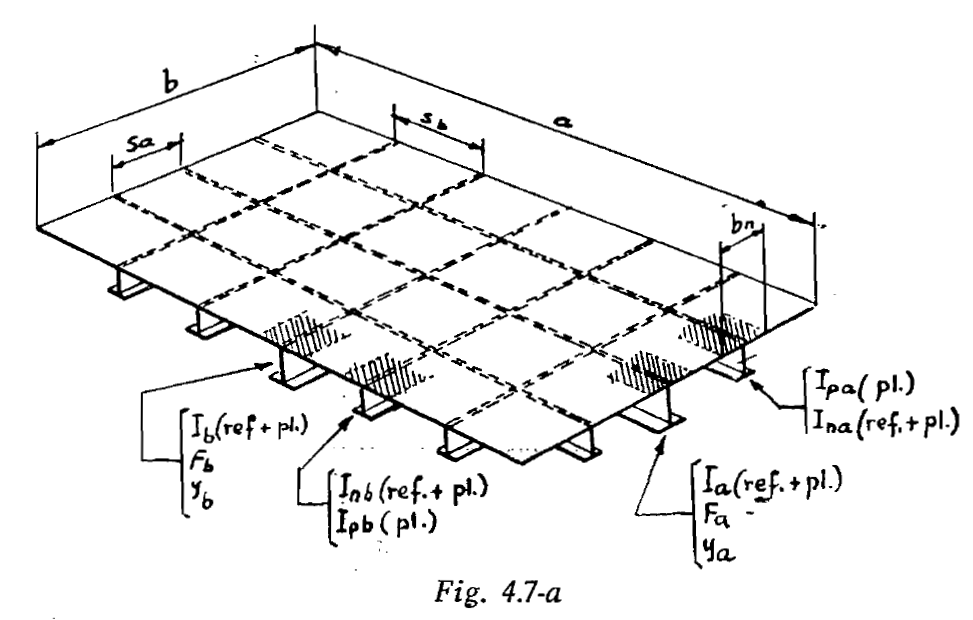
\includegraphics[width=.7\textwidth]{fig/placaschade.png}
	\caption{Largo de placa longitudinal $a=\SI{26000}{\milli \meter}$. Ancho de placa transversal $b=\SI{8800}{\milli\meter}$. Espesor de placa doble fondo $t=7\si{\milli \meter}$.}
	\label{fig:placaschade}
\end{figure}

Se va plantear el siguiente esquema para llegar a un número que se aproxime al resultado obtenido.
\begin{itemize}
	\item $I_{varenga}= \SI{1,267e9}{\milli \meter^4}$
	\item $I_{vagra}=\SI{6,336e9}{\milli \meter ^4}$
	\item $I_{bulbo}=\SI{4,572e5}{\milli \meter ^4}$
	\item $I_{\mathrm{pb}}= \frac{t^3 s_b}{12}=\SI{9,29e4}{\milli \meter^4} $
	\item $I_{\mathrm{pa}}= \frac{t^3 s_a}{12}=\SI{1,86e4}{\milli \meter^4} $
\end{itemize}
donde $s$ es la separación entre refuerzos. $s_b=3250\si{\milli \meter}$ y $s_a=650\si{\milli \meter}$ correspondiente a la distancia entre varengas. Por como se entiende las definiciones de \cite{dominguez1969calculo}:
\[
I_{\mathrm{b}}=I_{\mathrm{pb}}+I_{varenga}=\SI{1,267e9}{\milli \meter ^4}, \qquad I_{\mathrm{a}}=I_{\mathrm{pa}}+I_{vagra}=\SI{6,336e9}{\milli \meter ^4}
\]
\[
I_{\mathrm{nb}}=I_{\mathrm{pb}}+I_{varenga}=\SI{1,267e9}{\milli \meter ^4}, \qquad I_{\mathrm{na}}=I_{\mathrm{pa}}+I_{bulbo}=\SI{4,643e5}{\milli \meter ^4}
\]


\[
i_{a}=\frac{I_{\mathrm{n a}}}{s_{a}}+2\left(\frac{I_{\mathrm{a}}-I_{\mathrm{na}}}{b}\right)=\SI{2,88e6}{\milli \meter^3}, \qquad i_b = \frac{I_{\mathrm{n b}}}{s_{b}}+2\left(\frac{I_{\mathrm{b}}-I_{\mathrm{nb}}}{a}\right)=\SI{3,898e5}{\milli \meter^3}
\]

Los valores  $I_{\mathrm{pa}}$ y $I_{\mathrm{pb}}$ son los momentos de inercia del doble fondo longitudinal y transversal, respectivamente. Toma el ancho efectivo como la mitad del espaciamiento entre longitudinales.  

Estos valores se usan para calcular el coeficiente de torsión $\eta$ y la relación virtual de los lados del panel $\rho$, calculo que resulta trivial para justo este ejemplo donde no se tiene transversales.

\[
\rho=\frac{a}{b} \sqrt[4]{\frac{i_{b}}{i_{a}}}= 9.7
\]
\[
\eta=\sqrt{\frac{\mathrm{I}_{\mathrm{pa}}}{\mathrm{I}_{\mathrm{na}}} \cdot \frac{\mathrm{I}_{\mathrm{pb}}}{\mathrm{I}_{\mathrm{nb}}}} = 5,4\times 10^{-4} \approx 0
\]

Procedemos a buscar el valor de $K$ en las curvas de Schade. Los valores de tabla para desplazamientos en el centro de la \textbf{placa simplemente apoyada} de material con modulo Poisson $0,3$, resultan ser
\[
K_w=0,013  
\] 

Por ultimo queda calcular el desplazamiento usando la igualdad teniendo en cuenta unidades en $\frac{\si{\newton}}{\si{\milli \meter}}$ y $\si{\milli \meter}$.

\[
w = K_w \cdot \frac{ p b^4  }{E i_b} = \SI{4,88}{\milli \meter}
\]

El resultado de Schade no dá el desplazamiento máximo obtenido en la simulación de NX pero sí da muy parecido al desplazamiento sobre la mitad de la placa, sobre el \emph{refuerzo longitudinal central}.


\section{Conclusión}
El resultado predispone de buenas características. Se pueden observar campos de tensiones en el doble fondo (figura \ref{fig:optimizacion}) similares a la de una placa empotrada (figura \ref{fig:VMempotrado}). Se tiene también un pequeño relieve de tensiones en su cara central. Esto se debe a que los longitudinales aportan un pequeño giro a la placa al deformarse. Se tiene entonces una superposición con el caso mencionado anteriormente, y el estado de tensiones de una placa simplemente apoyada (figura \ref{fig:VMapoyado}).


Los resultados de la optimización indican que se puede ahorrar una gran cantidad de material. Si suponemos que el sistema tiene dimensiones proporcionales al buque estudiado entonces se ahorra un 34\% de material en planchas, sin considerar la reducción en tamaño de los perfiles bulbos. Mientras que el fondo y las vagras se redujeron en 50\% el doble fondo solo se redujo en 30\%. Esto se debe a que las deformaciones sobre el doble fondo son altas por la presión hidrostática. Agregar más hileras de longitudinales reduce este efecto. Se vuelve complejo optimizar el doble fondo agregando longitudinales y intentando de ahorrar costos. 

Llegado al punto anterior la opción más práctica sería agregar transversales  y así reducir el material de las varengas, cuyo espesor se mantuvo igual durante la optimización por las razones mencionadas en la sección de optimización.

Dicho esto último hay mucha libertad en como optimizar la estructura de doble fondo, libertades consideradas en software de cálculo de estructuras de buques y que exceden el alcance de este informe que fue hecho para la materia de grado Elementos Finitos II - 31.92 de el Instituto Tecnológico de Buenos Aires.

\clearpage
\bibliography{labibliografia} % Indica archivo
\bibliographystyle{plainnat} 

\end{document}